\section{Apache Hadoop}
\label{sec:hadoop}

Apache\texttrademark Hadoop\textregistered ist ein in Java entwickeltes Open"=Source"=Software"=Projekt, welches die Verarbeitung von großen Datenmengen auf einem verteilten System ermöglicht.
Hadoop wird federführend von der \emph{Apache Foundation} entwickelt und enthält verschiedene vollständig skalierbare Komponenten \cite{HadoopHomePage}.
Dadurch wird ermöglicht, ein Hadoop"=Cluster auf nur einem einzelnen PC, aber auch verteilt auf zahlreichen Servern auszuführen, auf dem wiederum Anwendungen zum Verarbeiten von großen Datenmengen ausgeführt werden können.
Die dem Cluster und den Anwendungen verfügbaren Ressourcen beschränken sich lediglich auf die Summe der verfügbaren Ressourcen aller Hosts, auf denen das Cluster ausgeführt wird.
Hadoop besitzt hierzu folgende Kernmodule \cite{HadoopHomePage}:

\begin{description}
	\item[Hadoop Common] \hfill \\
        Gemeinsam genutzte Kernkomponenten
	\item[Hadoop \acrshort{YARN} (\acrlong{YARN}\glsunset{YARN})] \hfill \\
        Framework zur Verteilung und Ausführung von Anwendungen und das dazugehörige Ressourcen"=Management
	\item[\acrlong{HDFS} (\acrshort{HDFS}\glsunset{HDFS})] \hfill \\
        Verteiltes Dateisystem zum Speichern von Daten auf dem Cluster
	\item[Hadoop \gls{MR}] \hfill \\
        Implementierung des \gls{MR}"=Ansatzes zum Verarbeiten von großen Datenmengen, nutzt YARN zur Ausführung der Anwendungen
\end{description}

Aufgrund seiner Verbreitung stellt Hadoop eine der wichtigsten Implementierungen des \gls{MR}"=Ansatzes dar \cite{PoweredByHadoop}.
Die Ein"= und Ausgabedaten sind hierbei als \emph{Key"=Value}"=Paare definiert, die mithilfe des \gls{MR}"=Frameworks verarbeitet werden.
Hierbei werden zunächst die eingelesenen Eingabedaten in kleine und dadurch einfach zu verarbeitende Datenmengen aufgeteilt.
Die geteilten Daten werden dann in mehreren, parallel ausgeführten Map"=Tasks verarbeitet und zwischengespeichert.
Die zwischengespeicherten Daten werden anschließend von einem oder mehreren Reduce"=Tasks zusammengeführt und in die Ausgabedateien geschrieben.
Das Framework besitzt eine hohe Fehlertoleranz, da ein fehlerhafter Task jederzeit neu gestartet werden kann \cite{Dean2004,Dean2010}.
Zur Speicherung der Ein-, Zwischen- und Ausgabedaten wird im Falle von Hadoop das HDFS genutzt \cite{HadoopMapRedTutorial271}.
Für eine ausführliche Beschreibung des \gls{MR}"=Frameworks sei hier auf \cite{Dean2004} und \cite{Dean2010} verwiesen; eine generelle Betrachtung des \gls{MR}"=Frameworks mit Vorteilen und möglichen Problemen lässt sich in \cite{Lee2012} finden.

Da das \gls{MR}"=Framework bzw. seine Implementierung in Hadoop nicht immer optimal genutzt werden kann und in der Praxis daher zum Teil auch zweckentfremdet wurde, wurde in \cite{Vavilapalli2013} das YARN"=Framework vorgestellt.
Die Kernidee ist hierbei die Trennung von Ressourcenmanagement und Scheduling vom eigentlichen Programm.
In diesem Kontext bildet der \gls{MR}"=Ansatz eine mögliche Anwendung, die mithilfe des YARN"=Frameworks ausgeführt wird \cite{Vavilapalli2013}.

Ein Hadoop"=Cluster mit dem YARN"=Framework besteht aus zwei wesentlichen Komponenten, dem \emph{Controller} mit \gls{RM} und den angeschlossenen \emph{Nodes}:

\begin{figure}[h]
    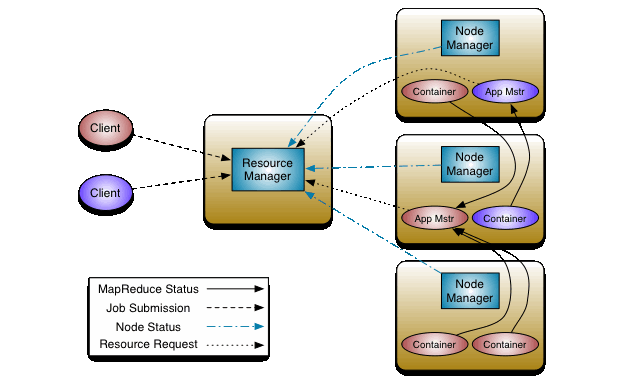
\includegraphics{./resources/yarn_architecture.png}
    \caption[Architektur des YARN"=Frameworks]
    {Architektur des YARN"=Frameworks (entnommen aus \cite{HadoopYarnArch271})}
    \label{fig:yarnarch}
\end{figure}

Der \gls{RM} dient hierbei als \emph{Load"=Balancer} für das gesamte Cluster und besteht aus dem \gls{AM} und dem \emph{Scheduler}, die eigentliche Ausführung der Anwendungen findet auf den Nodes statt.
Der \gls{AM} ist für die Annahme und Ausführung von einzelnen Anwendungen zuständig, denen der Scheduler die dafür notwendigen Ressourcen im Cluster zuteilt.
Jeder Node besitzt einen \gls{NM}, der für die Überwachung der Ressourcen auf dem jeweiligen Node sowie der auf dem Node ausgeführten YARN"=Container zuständig ist und diese Daten dem \gls{RM} übermittelt.

Jede YARN"=Anwendung bzw. Job besteht aus einer oder mehreren Ausführungsinstanzen, genannt \emph{Attempts}.
Jeder Attempt besitzt einen eigenen \gls{AppMstr}, der das Monitoring der Anwendung und die Kommunikation mit dem \gls{RM} und \gls{NM} durchführt und die dafür benötigten Daten bereitstellt \cite{HadoopYarnArch271}.
Die eigentliche Ausführung eines Tasks einer Anwendung findet in den bereits erwähnten \emph{Containern} statt, die jeweils einem Attempt zugeordnet sind.
Container können auf einem beliebigen Node ausgeführt werden und dienen der Ausführung eines Tasks der Anwendung.
Der \gls{AppMstr} wird hierbei ebenfalls in einem YARN"=Container ausgeführt.

Für die Fallstudie in dieser Masterarbeit ist zudem nicht unwesentlich, dass die Kommunikation zwischen den einzelnen Komponenten nicht in allen Fällen in Echtzeit stattfindet.
Vor allem das Prüfen des generellen Node"=Zustandes durch den \gls{RM} wird bei einer Standard"=Konfiguration in periodischen Abständen von jeweils mehreren Minuten durchgeführt.
Erst nachdem ein \gls{NM} nach mehreren Minuten keine Rückmeldung an den \gls{RM} sendet, wird der Node als defekt markiert.
Ähnlich verhält es sich bei Zustandsabfragen an die \gls{AppMstr} der Anwendungen \cite{HadoopYarnConfig271}.

Ein weiterer Bestandteil von Hadoop bzw. YARN ist der \gls{TLS}.
Er ist speziell dafür entwickelt, die Metadaten und Logs der YARN"=Anwendungen zu speichern und als Anwendungshistorie bereitzustellen \cite{HadoopYarnTlServer271}.

Zum Steuern des Clusters bzw. dem Monitoring der mithilfe von YARN ausgeführten Anwendungen stellt Hadoop drei Schnittstellen zur Verfügung.
Dies sind eine graphische Weboberfläche, was zugleich auch die wichtigste Schnittstelle darstellt, entsprechende Befehle für die \acrlong{CLI} (engl. \emph{Command-line interface}, kurz \acrshort{CLI})\glsunset{CLI} sowie eine REST"=API.
Während sich die Weboberfläche zur menschlichen Interaktion oder zur Fehlersuche eignet, dienen die \gls{CLI}"=Befehle vor allem zum Steuern des Clusters und die REST"=API zur automatisierten Rückgabe der Daten des Clusters zur Nutzung in anderen Programmen \cite{HadoopClusterSetup271,HadoopYarnCmds271,HadoopRmApi271,HadoopNmApi271}.

\cref{fig:hdfsarch} zeigt die dem YARN"=Framework sehr ähnliche Architektur des HDFS, welche ebenfalls aus einem Controller und mehreren Nodes besteht.

\begin{figure}
    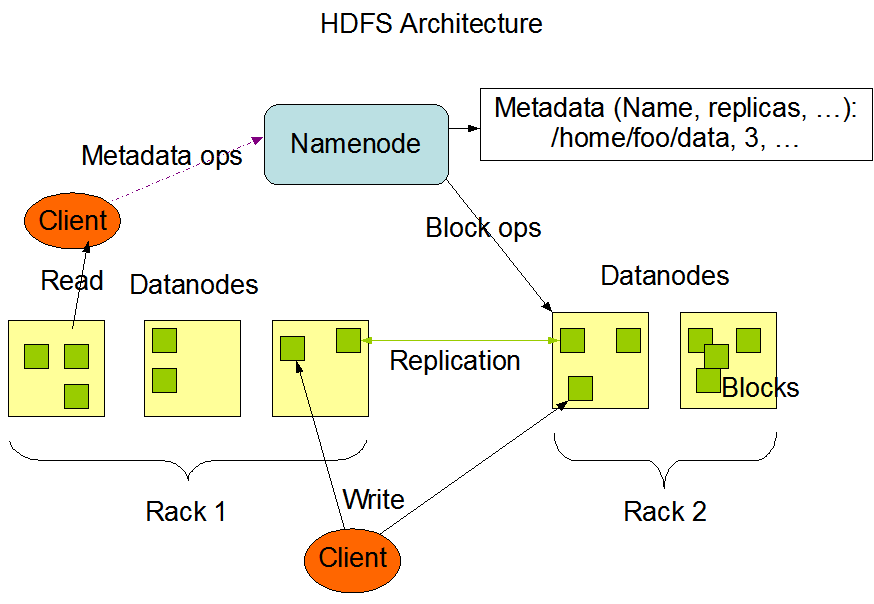
\includegraphics{./resources/hdfsarchitecture.png}
    \caption[Architektur des HDFS]
    {Architektur des HDFS (entnommen aus \cite{HadoopHdfsDesc271})}
    \label{fig:hdfsarch}
\end{figure}

Der \emph{NameNode} dient als Controller für die Verwaltung des Dateisystems und reguliert den Zugriff auf die darauf gespeicherten Daten.
Unterstützt wird er vom \emph{Secondary NameNode}, der Teile der internen Datenverwaltung des HDFS durchführt \cite{HadoopHdfsGuide271}.
Die Daten selbst werden in mehrere Blöcke aufgeteilt auf den \emph{DataNodes} gespeichert.
Um den Zugriff auf die Daten im Falle eines Node"=Ausfalls zu gewährleisten, wird jeder Block auf anderen Nodes repliziert.
Dateioperationen (wie Öffnen oder Schließen) werden direkt auf den DataNodes ausgeführt.
Sie sind darüber hinaus auch dafür verantwortlich, dass die gespeicherten Daten gelesen und beschrieben werden können \cite{Shvachko2010,HadoopHdfsDesc271}.

Das Überprüfen der DataNodes durch den NameNode erfolgt genauso wie bei den entsprechenden YARN"=Komponenten periodisch im Abstand von mehreren Minuten.
Auch hier dauert es bei einer Standard"=Konfiguration daher mehrere Minuten, bis ein DataNode als defekt markiert wird \cite{HadoopHdfsConfig271}.
